\section{Channel coding}
\subsection{Interleaving}
Since mostly error occur in bursts, it turned out that interleaving is good.
$$
\begin{array}{|cccccccc|}
\hline 1 & 7 & 13 & 19 & 25 & 31 & 37 & 43 \\
2 & 8 & 14 & 20 & 26 & 32 & 38 & 44 \\
3 & 9 & 15 & 21 & 27 & 33 & 39 & 45 \\
4 & 10 & 16 & 22 & 28 & 34 & 40 & 46 \\
5 & 11 & 17 & 23 & 29 & 35 & 41 & 47 \\
6 & 12 & 18 & 24 & 30 & 36 & 42 & 48 \\
\hline
\end{array}
$$
When one does interleaving and apply an error correction code again on the deinterleaved signal one can detect/correct much more errors since they are distributed to different regions.
\section{Trellis}
The goal of trellis modulation is to consider modulation and error correction in the same approach. Most trellis modulation approaches have one additional bit. Note, one does not increase the bandwidth or the bitrate. The mind distance and the min free path can be calculated with the folwoing formulas:
\begin{equation}
d_{\min }^2=\min _{k, l} d^2(k, l)
\end{equation}
\begin{equation}
d_{\text {free }}^2=\min _{\left\{a_k\right\} \neq\left\{a_k^{\prime}\right\}} \sum_k d^2\left(a_k, a_k^{\prime}\right)
\end{equation}
A good video can be found under the following \href{https://youtu.be/BcxmAph_DsE}{link}
\subsubsection{Example 2/3 4-PAM/8-PAM}\label{sbusubsec:example_pam}
Given is the following convolutional code for the last two bits, it can also be seen in \autoref{subfig:convolutional_code}:
\begin{itemize}
    \item K=3 Constraint length
    \item k=2 input bits
    \item n=3 output bits $\Rightarrow$ 2/3 Code
    \item g1= [1,1,1] generating vector of the code bits
    \item g2= [1,0,1] generating vector of the code bits
\end{itemize}
With this information one is then able to draw the set-partitioning as it can be seen in \autoref{subfig:set_partitioning}. There one looks that the most significant bit is always the furthest apart. The most significant bit is not coded.\newline
With this information, one can then draw the trellis, see also \autoref{subfig:trellis1}. When the state is [0,0] (storage element is [0,0]) and we insert the vector $x=\{x,0\}$ we stay in the same state, since the value from the storage does not change. Otherwise, when we insert the vector $x=\{x,1\}$ We change the state since the storage element is then [1,0]. With this, one can then draw the whole graph.\newline
To calculate the coding gain according to \autoref{eq:coding_gain} one has to calculate first the value of $d_{\text {min,uncoded }}^2$. For that, one can use the formula from \autoref{par:m-pam_power}, which says: $d_{\min }^2=\frac{12}{M^2-1}$. Duet to that $d_{\text {min,uncoded }}^2=\frac{4}{5}$ and $d_{\text {min,coded }}^2=\frac{4}{21}$. This means that A is $\sqrt{\frac{4}{21}}/2=\frac{\sqrt{21}}{21}$. The $d_{\text {free,coded }}^2$ can be searched with the trellis in \autoref{subfig:trellis2}. The distance is then $\left((7-3)^2+(7-5)^2+(7-3)^2\right)\cdot \left(\frac{\sqrt{21}}{21}\right)^2=\frac{12}{7}$. The gain is then $10\log_{10}(\frac{\frac{12}{7}}{\frac{4}{5}})=3.3dB$, due to the fact that the gain can be described with the following formula:

$$
G=\frac{d_{\text {free,coded }}^2}{d_{\text {min,uncoded }}^2}
$$
\begin{figure}[hbt!]
    \begin{subfigure}[t]{0.49\linewidth}
        \includegraphics[width=1\textwidth]{images/trellis/trellis_example1.jpg}
        \caption{convolutional code}\label{subfig:convolutional_code}
    \end{subfigure}
    \hfil
    \begin{subfigure}[t]{0.49\linewidth}
        \centering
        \includegraphics[width=0.6\textwidth]{images/trellis/trellis_example2.jpg}
        \caption{trellis1}\label{subfig:trellis1}
    \end{subfigure}
    \begin{subfigure}[t]{0.49\linewidth}
        \includegraphics[width=1\textwidth]{images/trellis/trellis_example3.jpg}
        \caption{trellis2}\label{subfig:trellis2}
    \end{subfigure}
    \hfil
    \begin{subfigure}[t]{0.4\linewidth}
        \includegraphics[width=1\textwidth]{images/trellis/trellis_example4.jpg}
        \caption{$d_{\text {free,coded }}^2$}\label{subfig:free_coded}
    \end{subfigure}
    \centering
    \begin{subfigure}[t]{0.49\linewidth}
        \includegraphics[width=1\textwidth]{images/trellis/trellis_example5.jpg}
        \caption{set-partitoning}\label{subfig:set_partitioning}
    \end{subfigure}
\caption{trellis}
\label{fig:ex_trellis}
\end{figure}
\FloatBarrier 
\subsubsection{1/2 QPSK TCM}
1/2 mans one has one input and two outputs.
\begin{equation}
    \begin{array}{rrrrrr}
    \hline \tilde{m} & \text { number of states } & m & \text { rate } & \text { constellation } & \text { asympt. gain } G \\
    \hline 1 & 2 & 1 & 1 / 2 & \text { BPSK/QPSK } & 1.76 \mathrm{~dB} \\
    1 & 2 & 2 & 2 / 3 & \text { QPSK/8-PSK } & 1.1 \mathrm{~dB}  \\
    1 & 4 & 2 & 2 / 3 & \text { QPSK/8-PSK } & 3.0 \mathrm{~dB}   \\
    2 & 8 & 2 & 2 / 3 & \text { QPSK/8-PSK } & 3.6 \mathrm{~dB}   \\
    2 & 8 & 3 & 3 / 4 & 8 \text {-PSK/16-PSK } & 3.98 \mathrm{~dB}  \\
    \hline
    \end{array}
\end{equation}
\subsubsection{Function}
The number of states of a trellis is always given by two to the power of number of storage elements, for example \autoref{fig:pdf2} has two states, since $2^1=2$. The coding gain G is given by \autoref{eq:coding_gain}.
\begin{equation}\label{eq:coding_gain}
G=\frac{d_{\text {free,coded }}^2}{d_{\text {min,uncoded }}^2}
\end{equation}
When one wants to calculate the coding gain for a two-state 2/3 TCM with QPSK one gets the following result:
$$
G=\frac{2.5858}{2}=1.2929=1.12 \mathrm{~dB}
$$
This is because the shortest distance squared in QPSK is 2, see also \autoref{fig:shortest_path1}, when one sends one bit the shortest distance squared is two, since one would go from position zero to position two in \autoref{fig:shortest_path1}. In a two-state 2/3 TCM it looks different, one has a storage element, due to that the signal looks like in \autoref{fig:shortest_path2} when one changes the LSB. This results in a total distance of $d_{\text {free }}^2=d^2(0,2)+d^2(0,1)=2+(2-\sqrt{2})=2.5858$ (Note to calculate the distance one always refers to zero as it is also done in \autoref{sbusubsec:example_pam}). When one would change the most significant bit the distance would be even higher, since one jumps always to the other side of the circle. 
\begin{figure}[ht]
    \begin{subfigure}[t]{0.3\linewidth}
        \resizebox{1\textwidth}{!}{\subimport{images/}{trellis1.tex}}
        \caption{state 0}\label{subfig:qpsk}
    \end{subfigure}
 \hfil
    \begin{subfigure}[t]{0.3\linewidth}
        \resizebox{1\textwidth}{!}{\subimport{images/}{trellis2.tex}}
        \caption{state 1}\label{subfig:8-psk}
    \end{subfigure}
    
\caption{QPSK shortest path}
\label{fig:shortest_path1}
\end{figure}
\begin{figure}[ht]
    \begin{subfigure}[t]{0.3\linewidth}
        \resizebox{1\textwidth}{!}{\subimport{images/}{trellis1.tex}}
        \caption{state 0}\label{subfig:qpsk}
    \end{subfigure}
    \hfil
    \begin{subfigure}[t]{0.3\linewidth}
        \resizebox{1\textwidth}{!}{\subimport{images/}{trellis2.tex}}
        \caption{state 1}\label{subfig:8-psk}
    \end{subfigure}
    \hfil
    \begin{subfigure}[t]{0.3\linewidth}
        \resizebox{1\textwidth}{!}{\subimport{images/}{trellis3.tex}}
        \caption{state 2}\label{subfig:8-psk}
    \end{subfigure}
    
\caption{two-state 2/3 TCM shortest path}
\label{fig:shortest_path2}
\end{figure}

\begin{figure}[ht]
    \centering
        %trim=left botm right top
        \includegraphics[page=135, clip, trim=6cm 17cm 4.5cm 7.5cm, width=0.8\textwidth]{data/99_TSM_SignProc LectureNotes 2022 part1.pdf}
    \caption{Minimum (squared) Euclidean distance in a constellation plot (unit circle) for 8-PSK.}
    \label{fig:pdf1}
\end{figure}
\begin{figure}[ht]
    \centering
        %trim=left botm right top
        \includegraphics[page=137, clip, trim=6cm 19cm 4.5cm 8.2cm, width=0.8\textwidth]{data/99_TSM_SignProc LectureNotes 2022 part1.pdf}
    \caption{Encoder for the constellation index for a two-state rate 2/3 TCM.}
    \label{fig:pdf2}
\end{figure}
\begin{figure}[ht]
    \centering
        %trim=left botm right top
        \includegraphics[page=137, clip, trim=5.5cm 10.5cm 4.5cm 15cm, width=0.8\textwidth]{data/99_TSM_SignProc LectureNotes 2022 part1.pdf}
    \caption{Trellis for a two-state rate $2 / 3$ TCM including parallel transitions, $\boldsymbol{y}=y_2 y_1 y_0$.}
    \label{fig:pdf3}
\end{figure}
\begin{figure}[ht]
    \centering
        %trim=left botm right top
        \includegraphics[width=0.8\textwidth]{images/trellis_example.jpg}
    \caption{Example}
    \label{fig:example_trellis}
\end{figure}

\subsubsection{Example two state 2/3 Trellis modulation}
See also the following \href{https://youtu.be/rnjy4_gXLAg}{video}. We have an input signal $x_1=\{0,1,0\}$ and $x_2=\{0,1,0\}$ and the received values are $n_1=0, n_2=-0.8+j, n_3=0$. We start at state zero and calculate now the distances to the other states. Since we received zero in the beginning, the squared distance  to zero is zero, to four four, to two two and to six also two. In the next state we received $-0.8+j$, therefore, the distance to zero is $(1--0.8)^2+(0-1)^2=4.24$, to point four $(-1--0.8)^2+(0-1)^2=1.04$, to point one $(\sqrt{2}--0.8)^2+(\sqrt{2}-1)^2=5.07$ and so on. for the last received signal one can do again the same. In the end one decides for the path which has the least squared distance, which is 0,6,1. This is also what was sent according to \autoref{tb:trellis}. The whole diagram can be found in \autoref{fig:example_trellis}
\begin{table}[h!]
\centering
 \begin{tabular}{||c c c c||} 
 \hline
 Bit & State1 & State2 & State3 \\ [0.5ex] 
 \hline\hline
 MSB & 0 & 1 & 0 \\ 
  & 0 & 1 & 0 \\
 LSB & 0 & 0 & 1 \\
 Result & 0 & 6 & 1 \\
 \hline
 \end{tabular}
 \label{tb:trellis}
 \end{table}
% \begin{figure}[ht]
%     \centering
%         %trim=left botm right top
%         \includegraphics[page=138, clip, trim=5cm 16.9cm 4.5cm 10cm, width=0.8\textwidth]{data/99_TSM_SignProc LectureNotes 2022 part1.pdf}
%     \caption{Encoder for a four-state rate 2/3 TCM.}
%     \label{fig:pdf4}
% \end{figure}
% \begin{figure}[ht]
%     \centering
%         %trim=left botm right top
%         \includegraphics[page=138, clip, trim=5.5cm 7cm 4.5cm 14cm, width=0.8\textwidth]{data/99_TSM_SignProc LectureNotes 2022 part1.pdf}
%     \caption{State diagram for a four-state TCM.}
%     \label{fig:pdf5}
% \end{figure}
% \begin{figure}[ht!]
%   \centering
%   \resizebox{0.8\textwidth}{!}{\subimport{images/}{trellis.tex}}
%   \caption{Trellis}
%   \label{fig:trellis}
% \end{figure}
\FloatBarrier 
\section{Modulation Variants}
entropy:
\begin{equation}
H(Y) \triangleq-\int_{-\infty}^{\infty} p(y) \log _2 p(y) d y
\end{equation}
conditional entrpy:
\begin{equation}
H(Y \mid X) \triangleq-\int_{-\infty}^{\infty} p(x) \int_{-\infty}^{\infty} p(y \mid x) \log _2 p(y \mid x) d y d x
\end{equation}
The capacity is then given as:
\begin{equation}
C=I(X ; Y)=H(Y)-H(Y \mid X)
\end{equation}
When one has a gaussian distributed signal and gausian distributet noise the max capacity is given with the formula below.
\begin{equation}
C=\frac{1}{2} \log _2\left(1+\frac{E_s}{\sigma^2}\right)
\end{equation}
For a discrete memoryless channel (DMC) the following applies.
\begin{equation}
C_{\mathrm{DMC}}=\max _{p(k)} \sum_{k=1}^K \sum_{j=1}^J p(j \mid k) p(k) \log _2 \frac{p(j \mid k)}{p(j)}
\end{equation}
where p(x) is the distribution for example zero and one with a dirac of 1/2 at each point.
Numerical evalution for the capacity.
\begin{equation}
=\frac{E_s}{\sigma^2} \log _2 \mathrm{e}-\frac{1}{\sqrt{2 \pi} \sigma} \mathrm{e}^{-\frac{E_s}{2 \sigma^2}} \int_{-\infty}^{\infty} \mathrm{e}^{-\frac{y^2}{2 \sigma^2}}\left(\cosh \frac{y \sqrt{E_s}}{\sigma^2}\right) \log _2\left(\cosh \frac{y \sqrt{E_s}}{\sigma^2}\right) d y .
\end{equation}

\begin{figure}[ht]

    \begin{subfigure}[t]{0.3\linewidth}
  \resizebox{1\textwidth}{!}{\subimport{images/}{QPSK.tex}}
\caption{QPSK}\label{subfig:qpsk}
    \end{subfigure}
 \hfil
    \begin{subfigure}[t]{0.3\linewidth}
\resizebox{1\textwidth}{!}{\subimport{images/}{8-PSK.tex}}
\caption{8-PSK}\label{subfig:8-psk}
    \end{subfigure}
\hfil
    \begin{subfigure}[t]{0.3\linewidth}
 \resizebox{1\textwidth}{!}{\subimport{images/}{16-PSK.tex}}
\caption{16-PSK}\label{subfig:16-psk}
    \end{subfigure}

    \begin{subfigure}[t]{0.3\linewidth}
\resizebox{1\textwidth}{!}{\subimport{images/}{16-QAM.tex}}
\caption{16-QAM}\label{subfig:16-qam}
    \end{subfigure}
    \hfil
    \begin{subfigure}[t]{0.69\linewidth}
\resizebox{1\textwidth}{!}{\subimport{images/}{m-pam.tex}}
\caption{8-PAM}\label{subfig:16-qam}
    \end{subfigure}
%
\caption{Constellation diagrams}
\end{figure}
\FloatBarrier 
\subsection{Symbol Energy, Bit Energy}
The average symbol and Bit energy in QAM and PSK is given by \autoref{eq:qam_psk_engergy}.
\begin{equation} \label{eq:qam_psk_engergy}
\begin{aligned}
& E_s=\frac{1}{M} \sum_{m=0}^{M-1}\left|\underline{s}_m\right|^2 \quad \frac{\text { Joules }}{\text { Symbol }} \\
& E_b=\frac{1}{\log_2(M)} E_s \quad \frac{\text { Joules }}{\text { bit }}
\end{aligned}
\end{equation}
Where:
\begin{itemize}
    \item M, is the number of points in the signal constellation. (for example in \autoref{fig:rectangular_quam} M=8)
    \item $\underline{s}_m$ one specific Symbol out of M
    \item $E_s$ ,is the average symbol energy
    \item $E_b$, is the average bit energy (it is divided by $\log_2(M)$ because with $2^M$ symbols one can transmit $M$ bits)
\end{itemize}
\FloatBarrier 
\subsubsection{Example Calculate bit and signal energy of M=8 rectangular QAM}
Given is the M=8 rectangular QAM that can be seen in \autoref{fig:rectangular_quam}
\begin{figure}[ht!]
  \centering
  \resizebox{8cm}{!}{\subimport{images/}{rectangular_quam.tex}}
  \caption{M=8 rectangular QAM for example}
  \label{fig:rectangular_quam}
\end{figure}
now one wants to calculate $E_s,E_b$. This can be done with \autoref{eq:qam_psk_engergy} this gives the following result (see also the following \href{https://youtu.be/Z3wHXSCrlSM}{video}).
$$
\begin{aligned}
E_s &=\frac{1}{M} \sum_{m=0}^{M-1}\left|\underline{s}_m\right|^2 \quad \frac{\text { Joules }}{\text { Symbol }}\\
& =\frac{1}{8}\left[\left(A^2+A^2\right) 4+\left((3 A)^2+A^2\right) 4\right] \\
& =\frac{1}{8}\left[8 A^2+40 A^2\right] \\
& =\frac{48}{8} A^2=6 A^2 \\
E_b & =\frac{6 A^2}{\log _2 8}=2 A^2
\end{aligned}
$$
Where:
\begin{itemize}
    \item A=Amplitude
\end{itemize}
\FloatBarrier 
\subsubsection{Example M-PAM/M-PSK based TCM}
\paragraph{Example derive the minimum Euclidean distance $d^2_{min}$ in an M-array PAM system, whose power has been normalized to one}\mbox{}\newline
\label{par:m-pam_power}
With \autoref{eq:qam_psk_engergy} one can calculate the energy per symbol (as a reference also have a look at \autoref{fig:m-pam}):
\begin{figure}[ht!]
  \centering
  \resizebox{10cm}{!}{\subimport{images/}{m-pam.tex}}
  \caption{M=8 PAM example}
  \label{fig:m-pam}
\end{figure}
$$
\begin{aligned}
E_s&=\frac{1}{M} \sum_{m=0}^{M-1}\left|\underline{s}_m\right|^2 \quad \frac{\text { Joules }}{\text { Symbol }}\\
& =\frac{1}{M} \cdot 2 \sum_{m=1}^{M / 2}((2 m-1) A)^2 \\
& =\frac{2 A^2}{M} \sum_{m=1}^{M / 2}(2 m-1)^2 \\
& =\frac{2 A^2}{M}\left(4 \sum_{m=1}^{M / 2} m^2-4 \sum_{m=1}^{M / 2} m+\sum_{m=1}^{M / 2} 1\right) \\
& =\frac{2 A^2}{M}\left(\frac{M(M+2)(M+1)}{6}-\frac{M(M+2)}{2}+\frac{M}{2}\right) \\
& =\frac{A^2}{3}\left(M^2-1\right)
\end{aligned}
$$
Since we want P = 1, we get
$$
A=\sqrt{\frac{3}{M^2-1}}
$$
Therefore 
$$
d_{\min }^2=(2\cdot A)^2=\frac{12}{M^2-1}
$$
\paragraph{Derive the general expression for the minimum Euclidean distance $d^2_{min}$ in an M-array PSK system}\mbox{}\newline
With \autoref{eq:qam_psk_engergy} one can calculate the energy per symbol
$$
\begin{aligned}
E_s&=\frac{1}{M} \sum_{m=0}^{M-1}\left|\underline{s}_m\right|^2 \quad \frac{\text { Joules }}{\text { Symbol }}\\
& =\frac{1}{M} \sum_{m=0}^{M}(A)^2\\
&=A^2
\end{aligned}
$$
Since we want P = 1, we get
$$
A=1
$$
\begin{figure}[ht]
\centering
    \begin{subfigure}[t]{0.3\linewidth}
        \resizebox{1\textwidth}{!}{\subimport{images/}{octagon.tex}}
        \caption{Octagon}\label{subfig:octagon}
    \end{subfigure}
 \hfil
 \centering
    \begin{subfigure}[t]{0.3\linewidth}
        \resizebox{1\textwidth}{!}{\subimport{images/}{triangle2.tex}}
        \caption{Triangle for cosine rule}\label{subfig:triangle2}
    \end{subfigure}
\caption{Help for cosine rule}
\label{fig:help_cosine_rule}
\end{figure}
% \begin{figure}[ht!]
%   \centering
%   \resizebox{6cm}{!}{\subimport{images/}{octagon.tex}}
%   \caption{Octagon}
%   \label{fig:octagon}
% \end{figure}
% \begin{figure}[ht!]
%   \centering
%   \resizebox{10cm}{!}{\subimport{images/}{triangle2.tex}}
%   \caption{Triangle for cosine rule}
%   \label{fig:triangle2}
% \end{figure}
\begin{equation}\label{eq:cosine_rule}
\cos (A)=\frac{b^2+c^2-a^2}{2 b c}
\end{equation}
With this and the cosine (\autoref{eq:cosine_rule}) rule one gets the following result (to get the idea with the cosine rule also have a look at \autoref{fig:help_cosine_rule}).
$$
\cos \left(\frac{2\cdot \pi}{M} \right)=\frac{2\cdot A^2-d^2_{min}}{2 \cdot A^2} \Rightarrow \cos \left(\frac{2\cdot \pi}{M} \right) \cdot 2 \cdot A^2 - 2 \cdot A^2=-d^2_{min} \Rightarrow d^2_{min}= 2 \cdot A^2 \left(1-\cos \left(\frac{2\cdot \pi}{M} \right)\right)=2 \left(1-\cos \left(\frac{2\cdot \pi}{M} \right)\right)
$$